
\phantomsection

% Increment the chapter counter so \thechapter shows the correct number
% and make it referenceable with \ref
\refstepcounter{chapter}

% Manually add this appendix to the Table of Contents
\addcontentsline{toc}{chapter}{Apéndice \thechapter: Búsqueda en bases de datos}

% Add vertical space above the title (mimics standard chapter spacing)
\vspace{40pt}

% Display the actual chapter title (centered, large, bold)
{\centering \normalfont\huge\bfseries Apéndice~\thechapter: Búsqueda en bases de datos~\par}

% Add spacing between title and horizontal rule
\vspace{10pt}

% Draw a horizontal line across the page for visual separation
{\centering \rule{\textwidth}{0.4pt} \par}

% Add vertical space between title section and content
\vspace{40pt}

% Set the running headers for left and right pages
\markboth{Apéndice \thechapter:Búsqueda en bases de datos}{Apéndice \thechapter: Búsqueda en bases de datos}



\FloatBarrier\section{Cadenas de búsqueda}\label{sec:cadenas-busqueda}


\begin{tcolorbox}[
		colback=gray!5,
		colframe=black!60,
		title=Cadena de búsqueda en ACM Full Text Collection,
		fonttitle=\bfseries,
		sharp corners=south
	]
	\scriptsize
	\begin{verbatim}
((HTCondor OR Condor) AND (HTC OR "High Throughput Computing" OR HPC OR "High
Performance Computing") AND (Universe OR "Execution Environment") AND (Project OR
Work) AND (Research OR Teaching OR Industry))
	\end{verbatim}
\end{tcolorbox}

\begin{tcolorbox}[
		colback=gray!5,
		colframe=black!60,
		title=Cadena de búsqueda en IEEE Xplore,
		fonttitle=\bfseries,
		sharp corners=south
	]
	\scriptsize
	\begin{verbatim}
(HTCondor OR Condor) AND (HTC OR (High Throughput Computing)) AND (Universe OR
(Runtime Environment)) AND (Research OR Teaching OR Industry)
	\end{verbatim}
\end{tcolorbox}

\begin{tcolorbox}[
		colback=gray!5,
		colframe=black!60,
		title=Cadena de búsqueda en Springer,
		fonttitle=\bfseries,
		sharp corners=south
	]
	\scriptsize
	\begin{verbatim}
((HTCondor — Condor) + (HTC — "High Throughput Computing" — HPC — "High
Performance Computing") + (Universe — "Execution Environment") + (Project — Work) +
(Research — Teaching — Industry))
	\end{verbatim}
\end{tcolorbox}

\begin{tcolorbox}[
		colback=gray!5,
		colframe=black!60,
		title=Cadena de búsqueda en ScienceDirect,
		fonttitle=\bfseries,
		sharp corners=south
	]
	\scriptsize
	\begin{verbatim}
(HTCondor OR Condor) (HTC OR "High Throughput Computing" OR HPC OR
"High Performance Computing") (Universe OR "Execution Environment")
(Project OR Work) (Research OR Teaching OR Industry)
	\end{verbatim}
\end{tcolorbox}

\begin{tcolorbox}[
		colback=gray!5,
		colframe=black!60,
		title=Cadena de búsqueda en Taylor \& Francis,
		fonttitle=\bfseries,
		sharp corners=south
	]
	\scriptsize
	\begin{verbatim}
(HTCondor OR Condor) AND (HTC OR (High Throughput Computing)) AND (Universe OR
(Runtime Environment)) AND (Research OR Teaching OR Industry)
  \end{verbatim}
\end{tcolorbox}


\section{Búsqueda de artículos sin criterios de inclusión/exclusión}\label{sec:busqueda-sin-criterios}

% ##### Imagenes de busqueda ########

\begin{figure}[H]
	\centering
	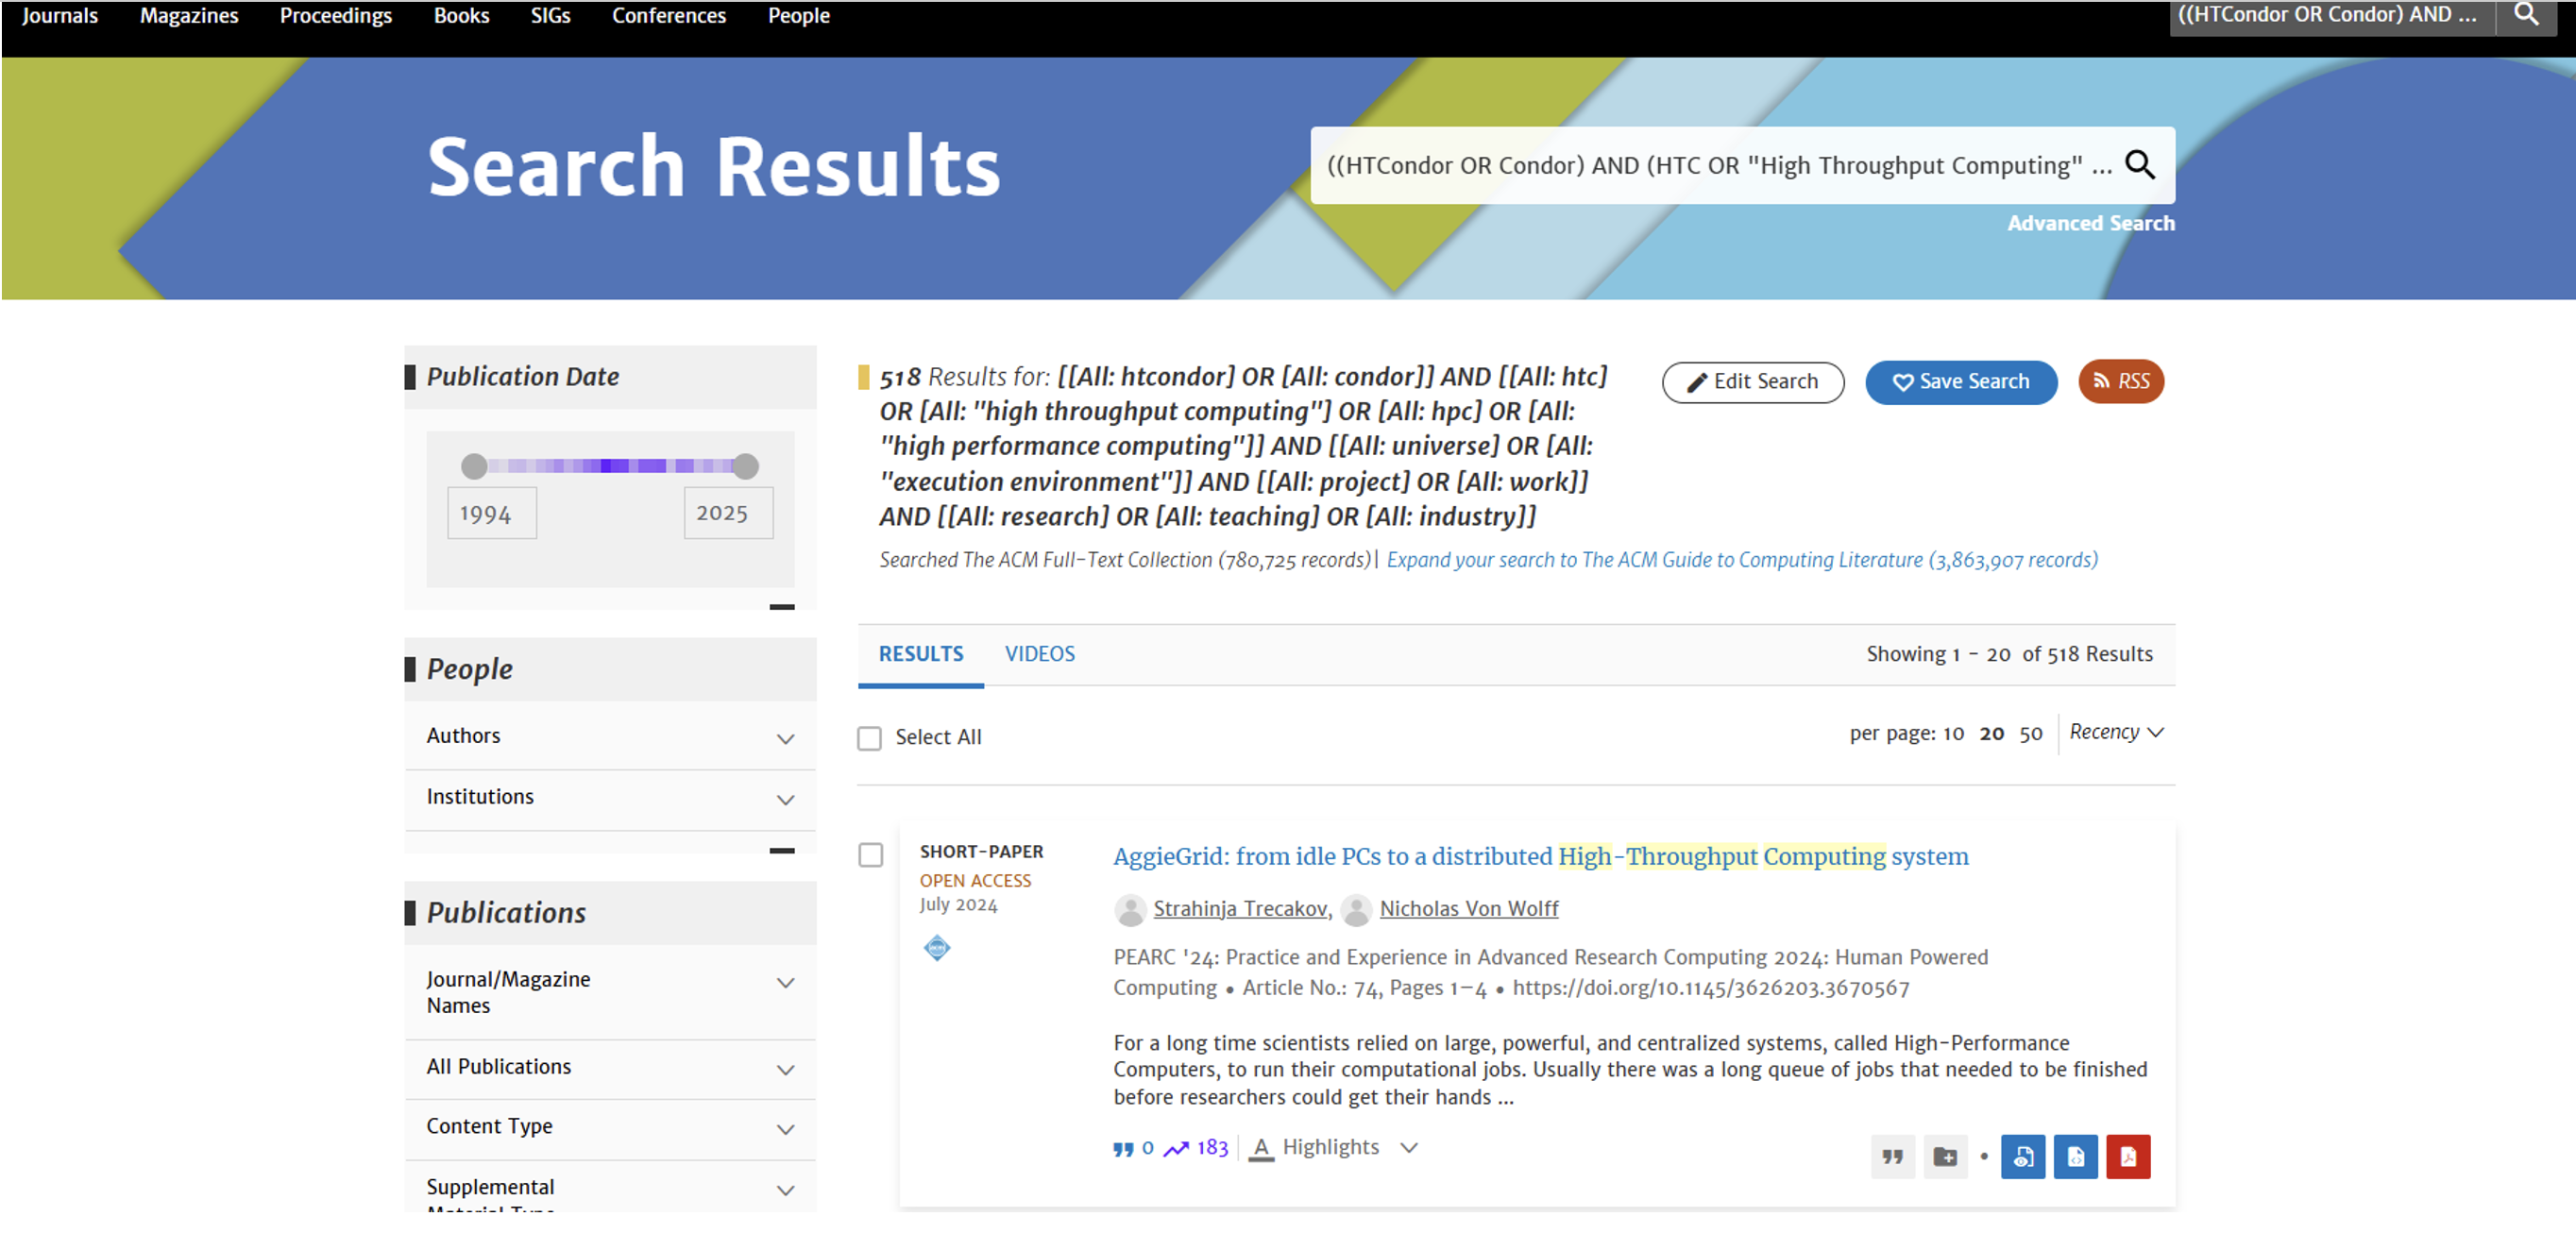
\includegraphics[width=\textwidth,keepaspectratio]{apendices/bases-datos/sin-exclusion/acm.png}
	\caption{Búsqueda de artículos de educación en ACM sin criterios de inclusión/exclusión \\
		Fecha de acceso: 12/03/25 9:13 pm
	}\label{fig:busqueda-acm-no-exclusion}
\end{figure}

\FloatBarrier

\begin{figure}[H]
	\centering
	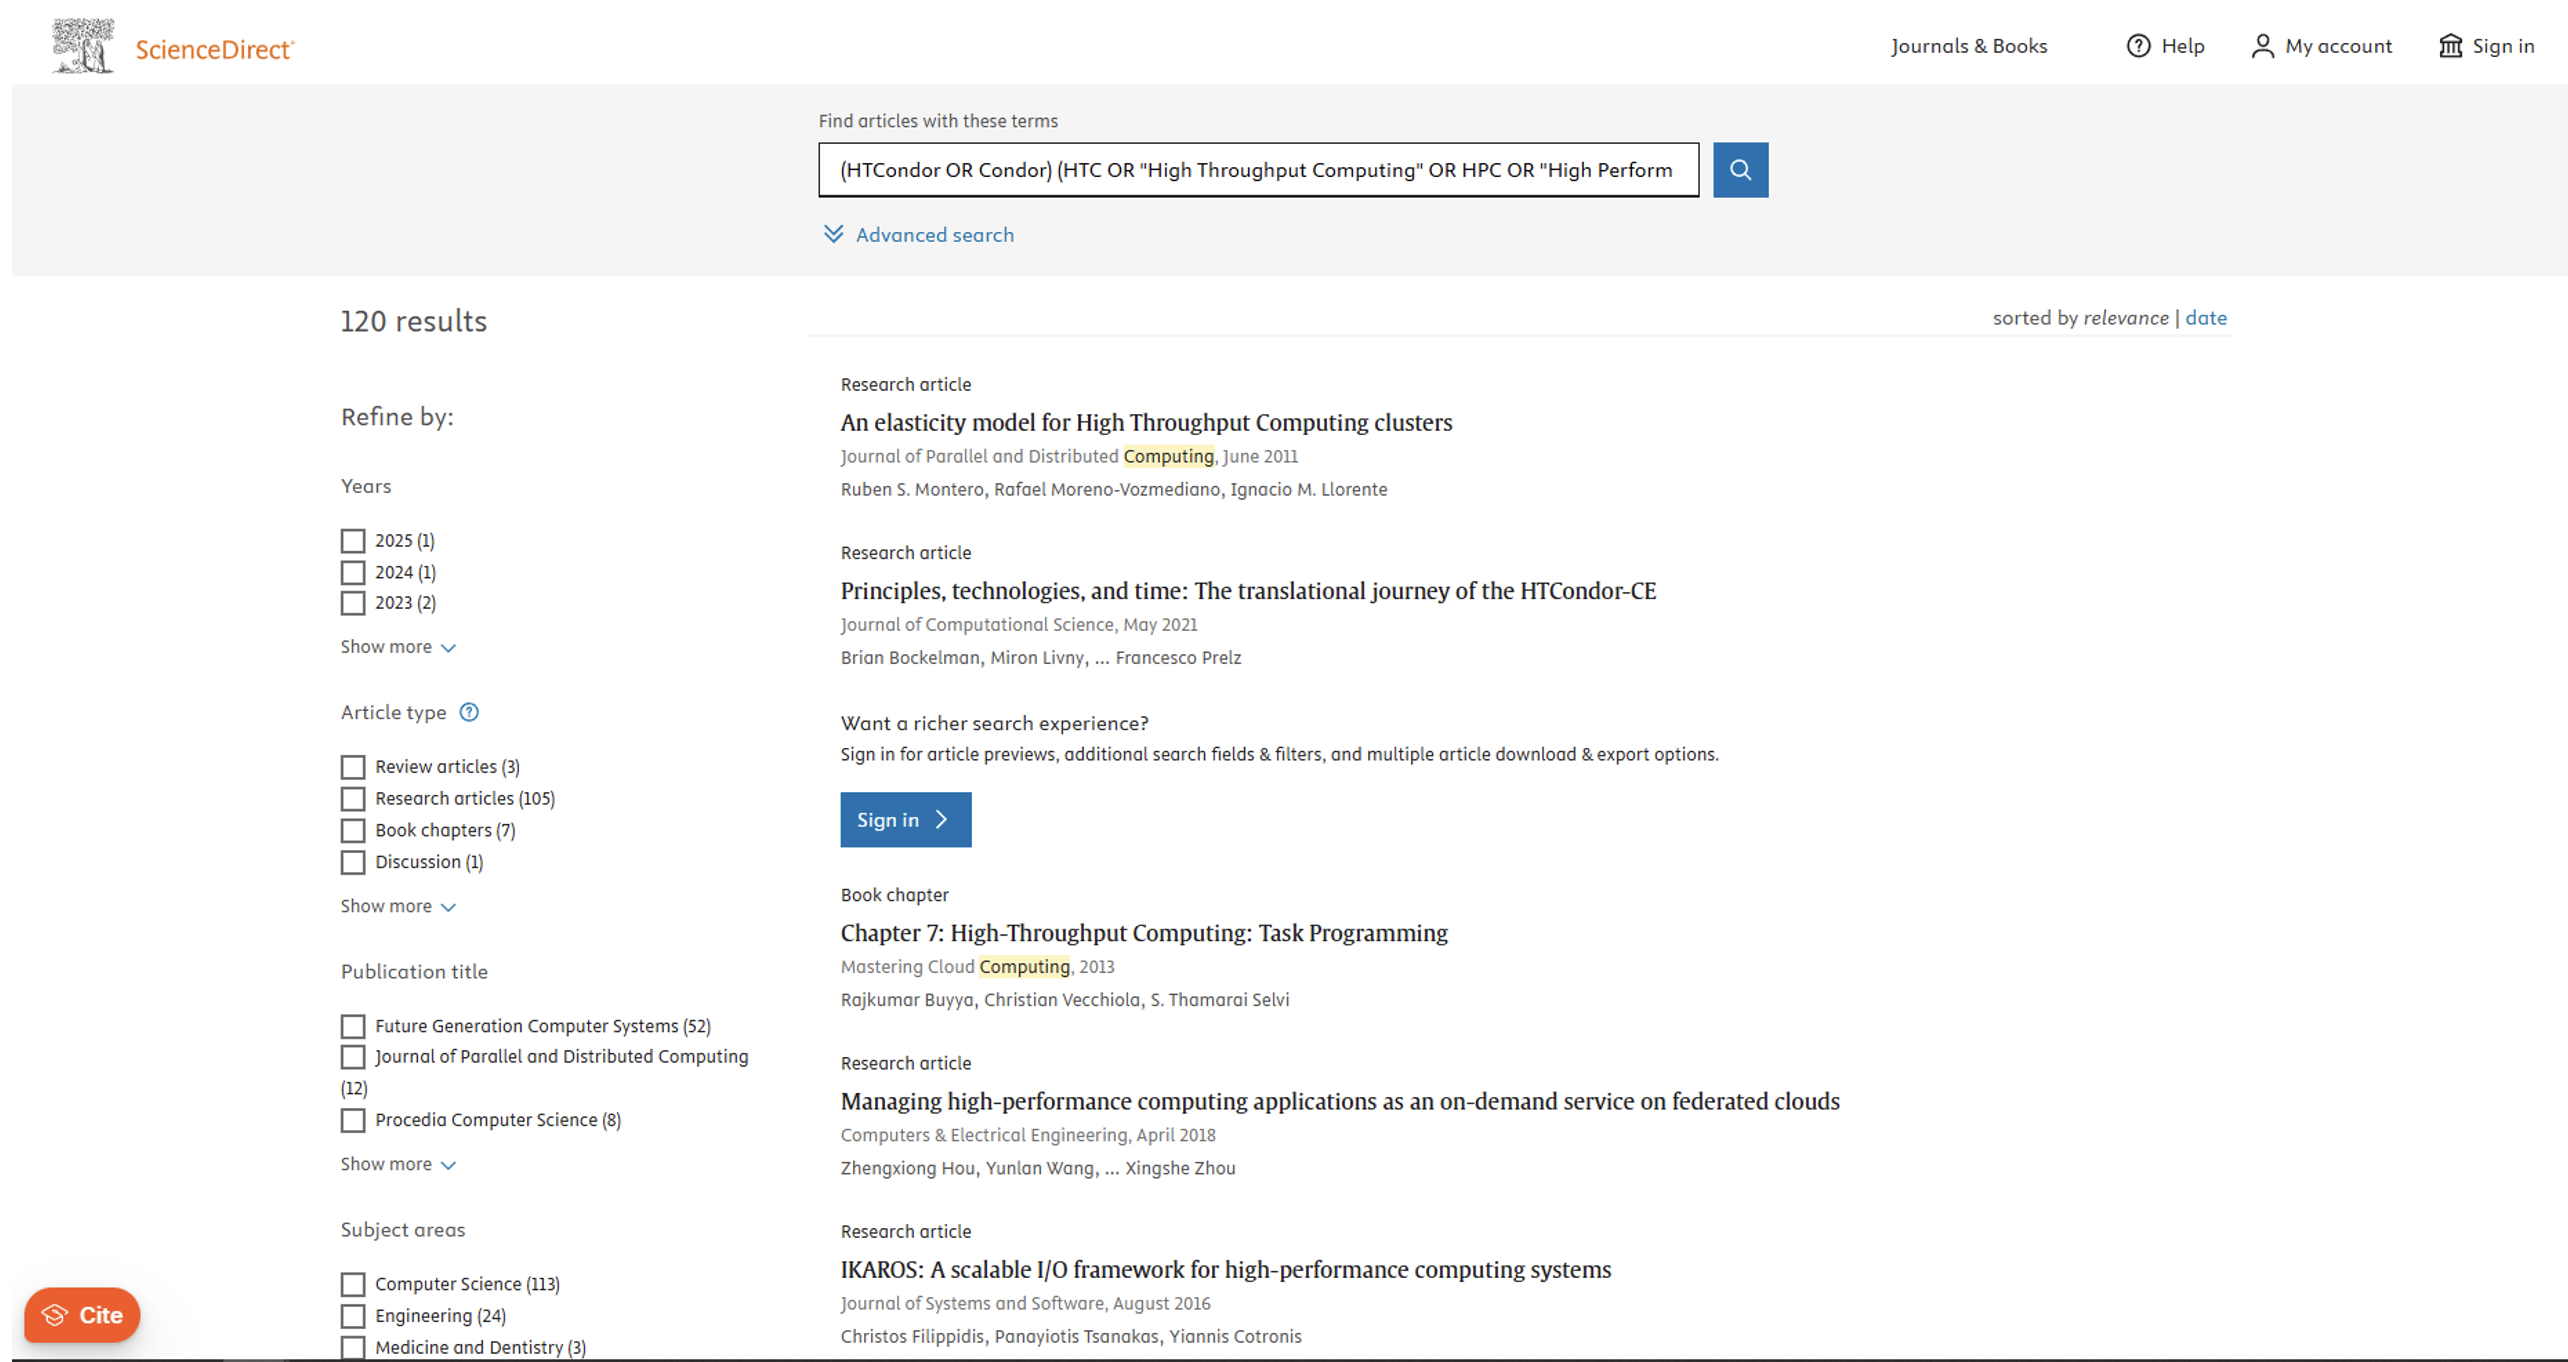
\includegraphics[width=\textwidth,keepaspectratio]{apendices/bases-datos/sin-exclusion/science-direct.png}
	\caption{Búsqueda de artículos de investigación en ACM sin criterios de inclusión/exclusión \\
		Fecha de acceso: 12/03/25 8:23 pm
	}\label{fig:busqueda-science-direct-no-exclusion}
\end{figure}

\begin{figure}[H]
	\centering
	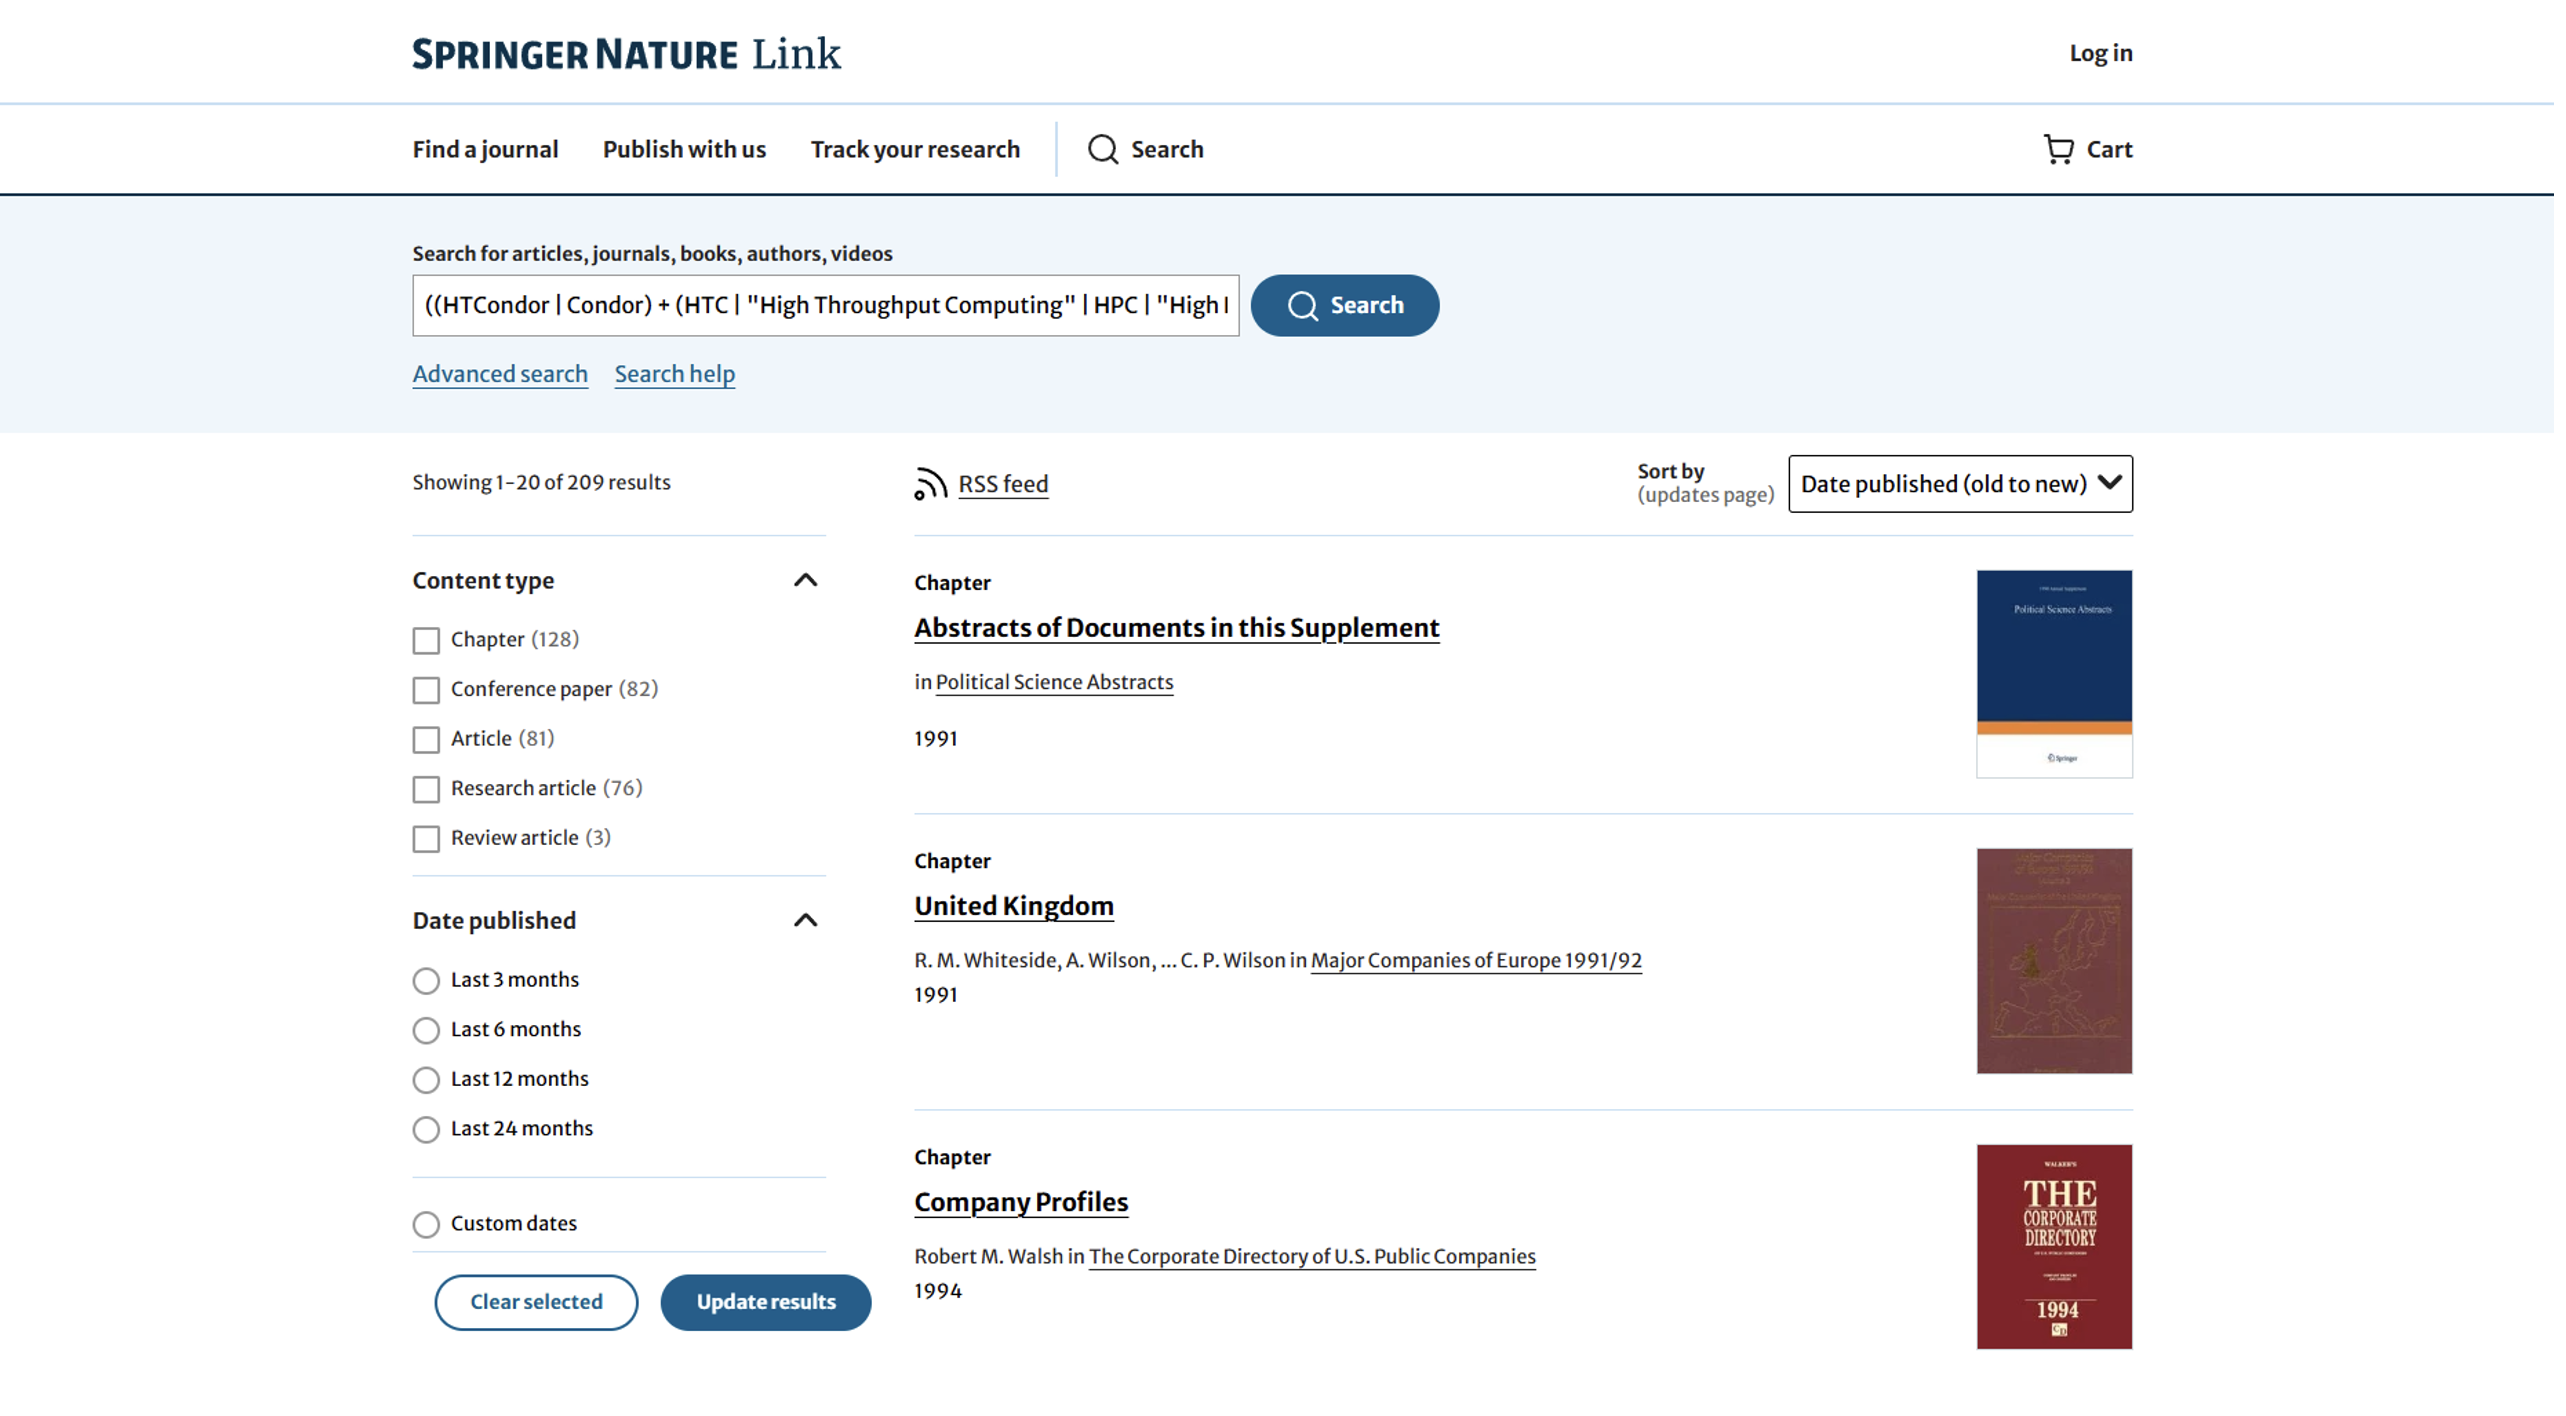
\includegraphics[width=\textwidth,keepaspectratio]{apendices/bases-datos/sin-exclusion/springer.png}
	\caption{Búsqueda de artículos de investigación en ACM sin criterios de inclusión/exclusión \\
		Fecha de acceso: 12/03/25 8:23 pm
	}\label{fig:busqueda-springer-no-exclusion}
\end{figure}


%########## Fin Imagenes %###################


\section{Búsqueda de artículos con criterios de inclusión/exclusión}\label{sec:busqueda-con-criterios}

\begin{figure}[H]
	\centering
	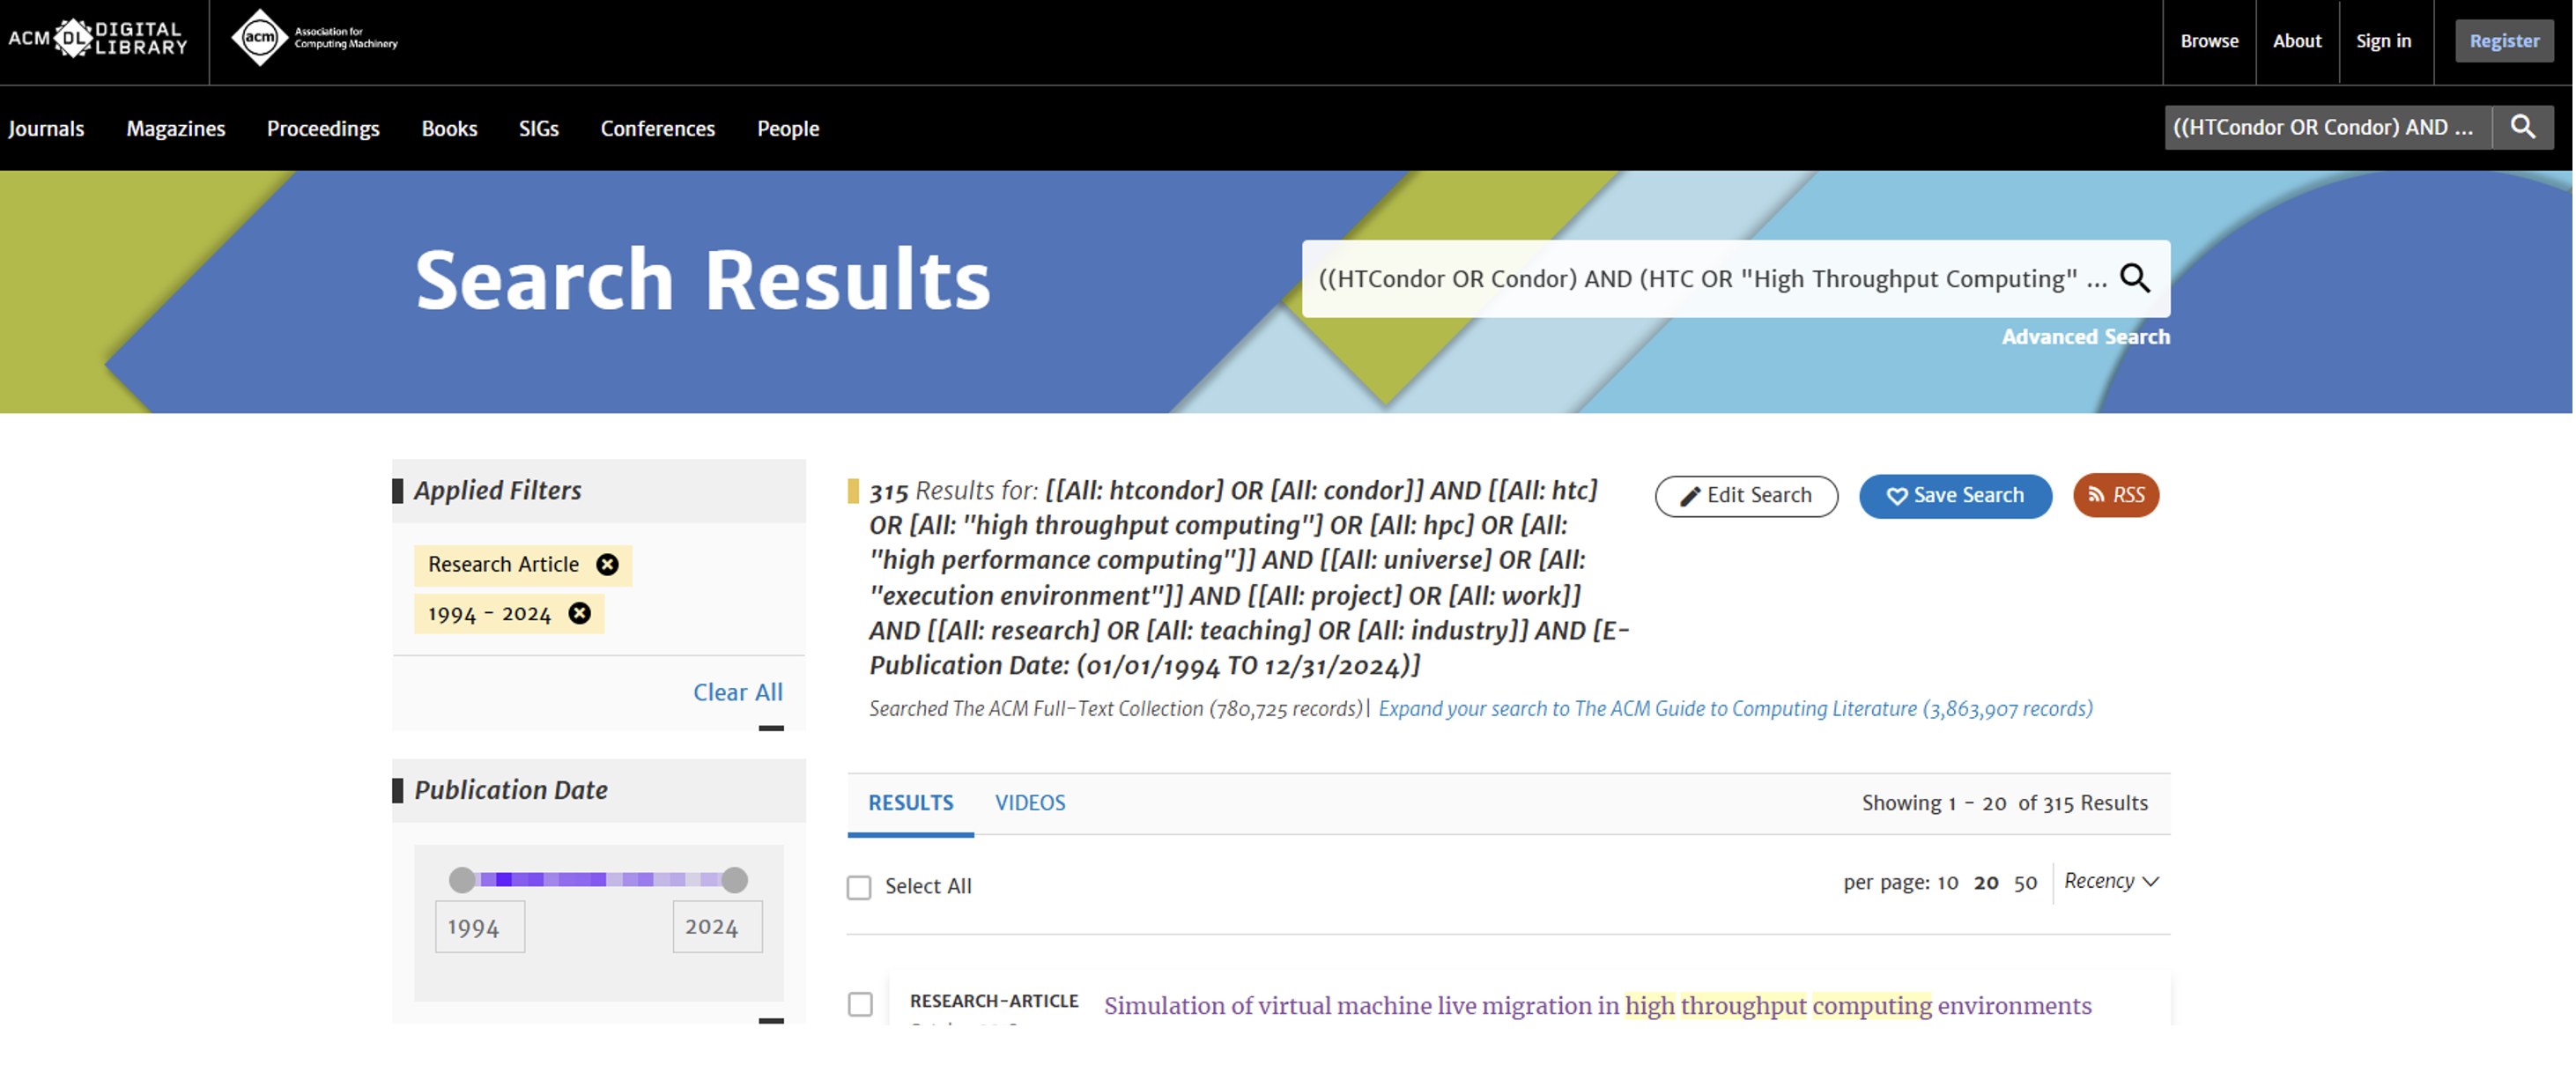
\includegraphics[width=\textwidth,keepaspectratio]{apendices/bases-datos/con-exclusion/acm.png}
	\caption{Búsqueda de artículos de educación en ACM sin criterios de inclusión/exclusión \\
		Fecha de acceso: 12/03/25 9:13 pm
	}\label{fig:busqueda-acm-con-exclusion}
\end{figure}

\FloatBarrier

\begin{figure}[H]
	\centering
	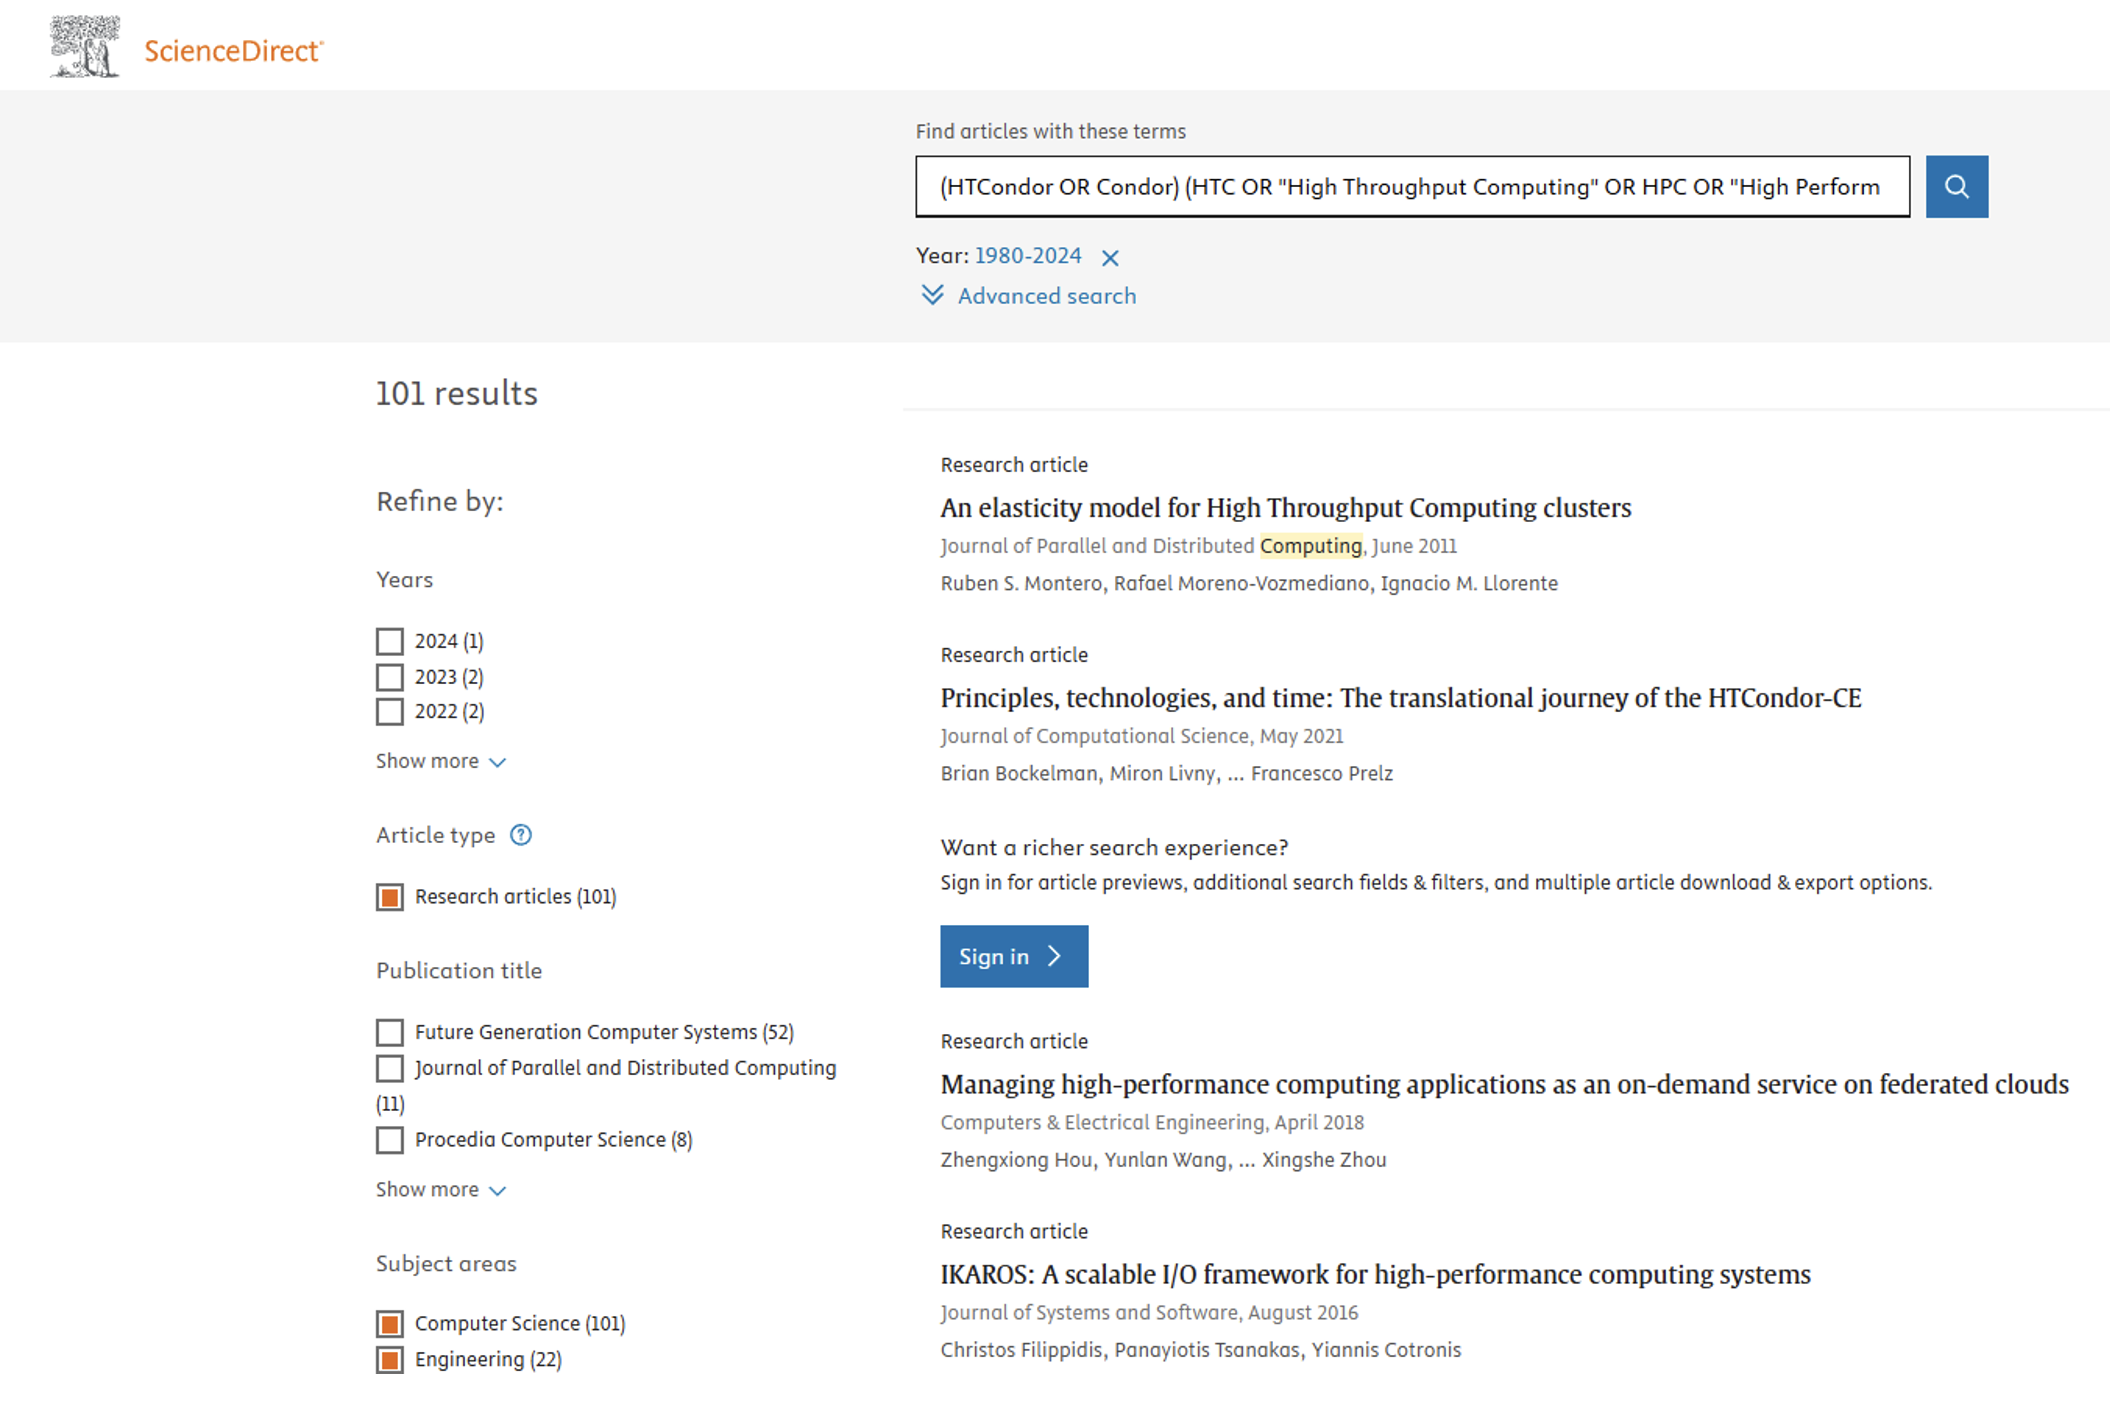
\includegraphics[width=\textwidth,keepaspectratio]{apendices/bases-datos/con-exclusion/science-direct.png}
	\caption{Búsqueda de artículos de investigación en ACM sin criterios de inclusión/exclusión \\
		Fecha de acceso: 12/03/25 8:23 pm
	}\label{fig:busqueda-science-direct-con-exclusion}
\end{figure}

\begin{figure}[H]
	\centering
	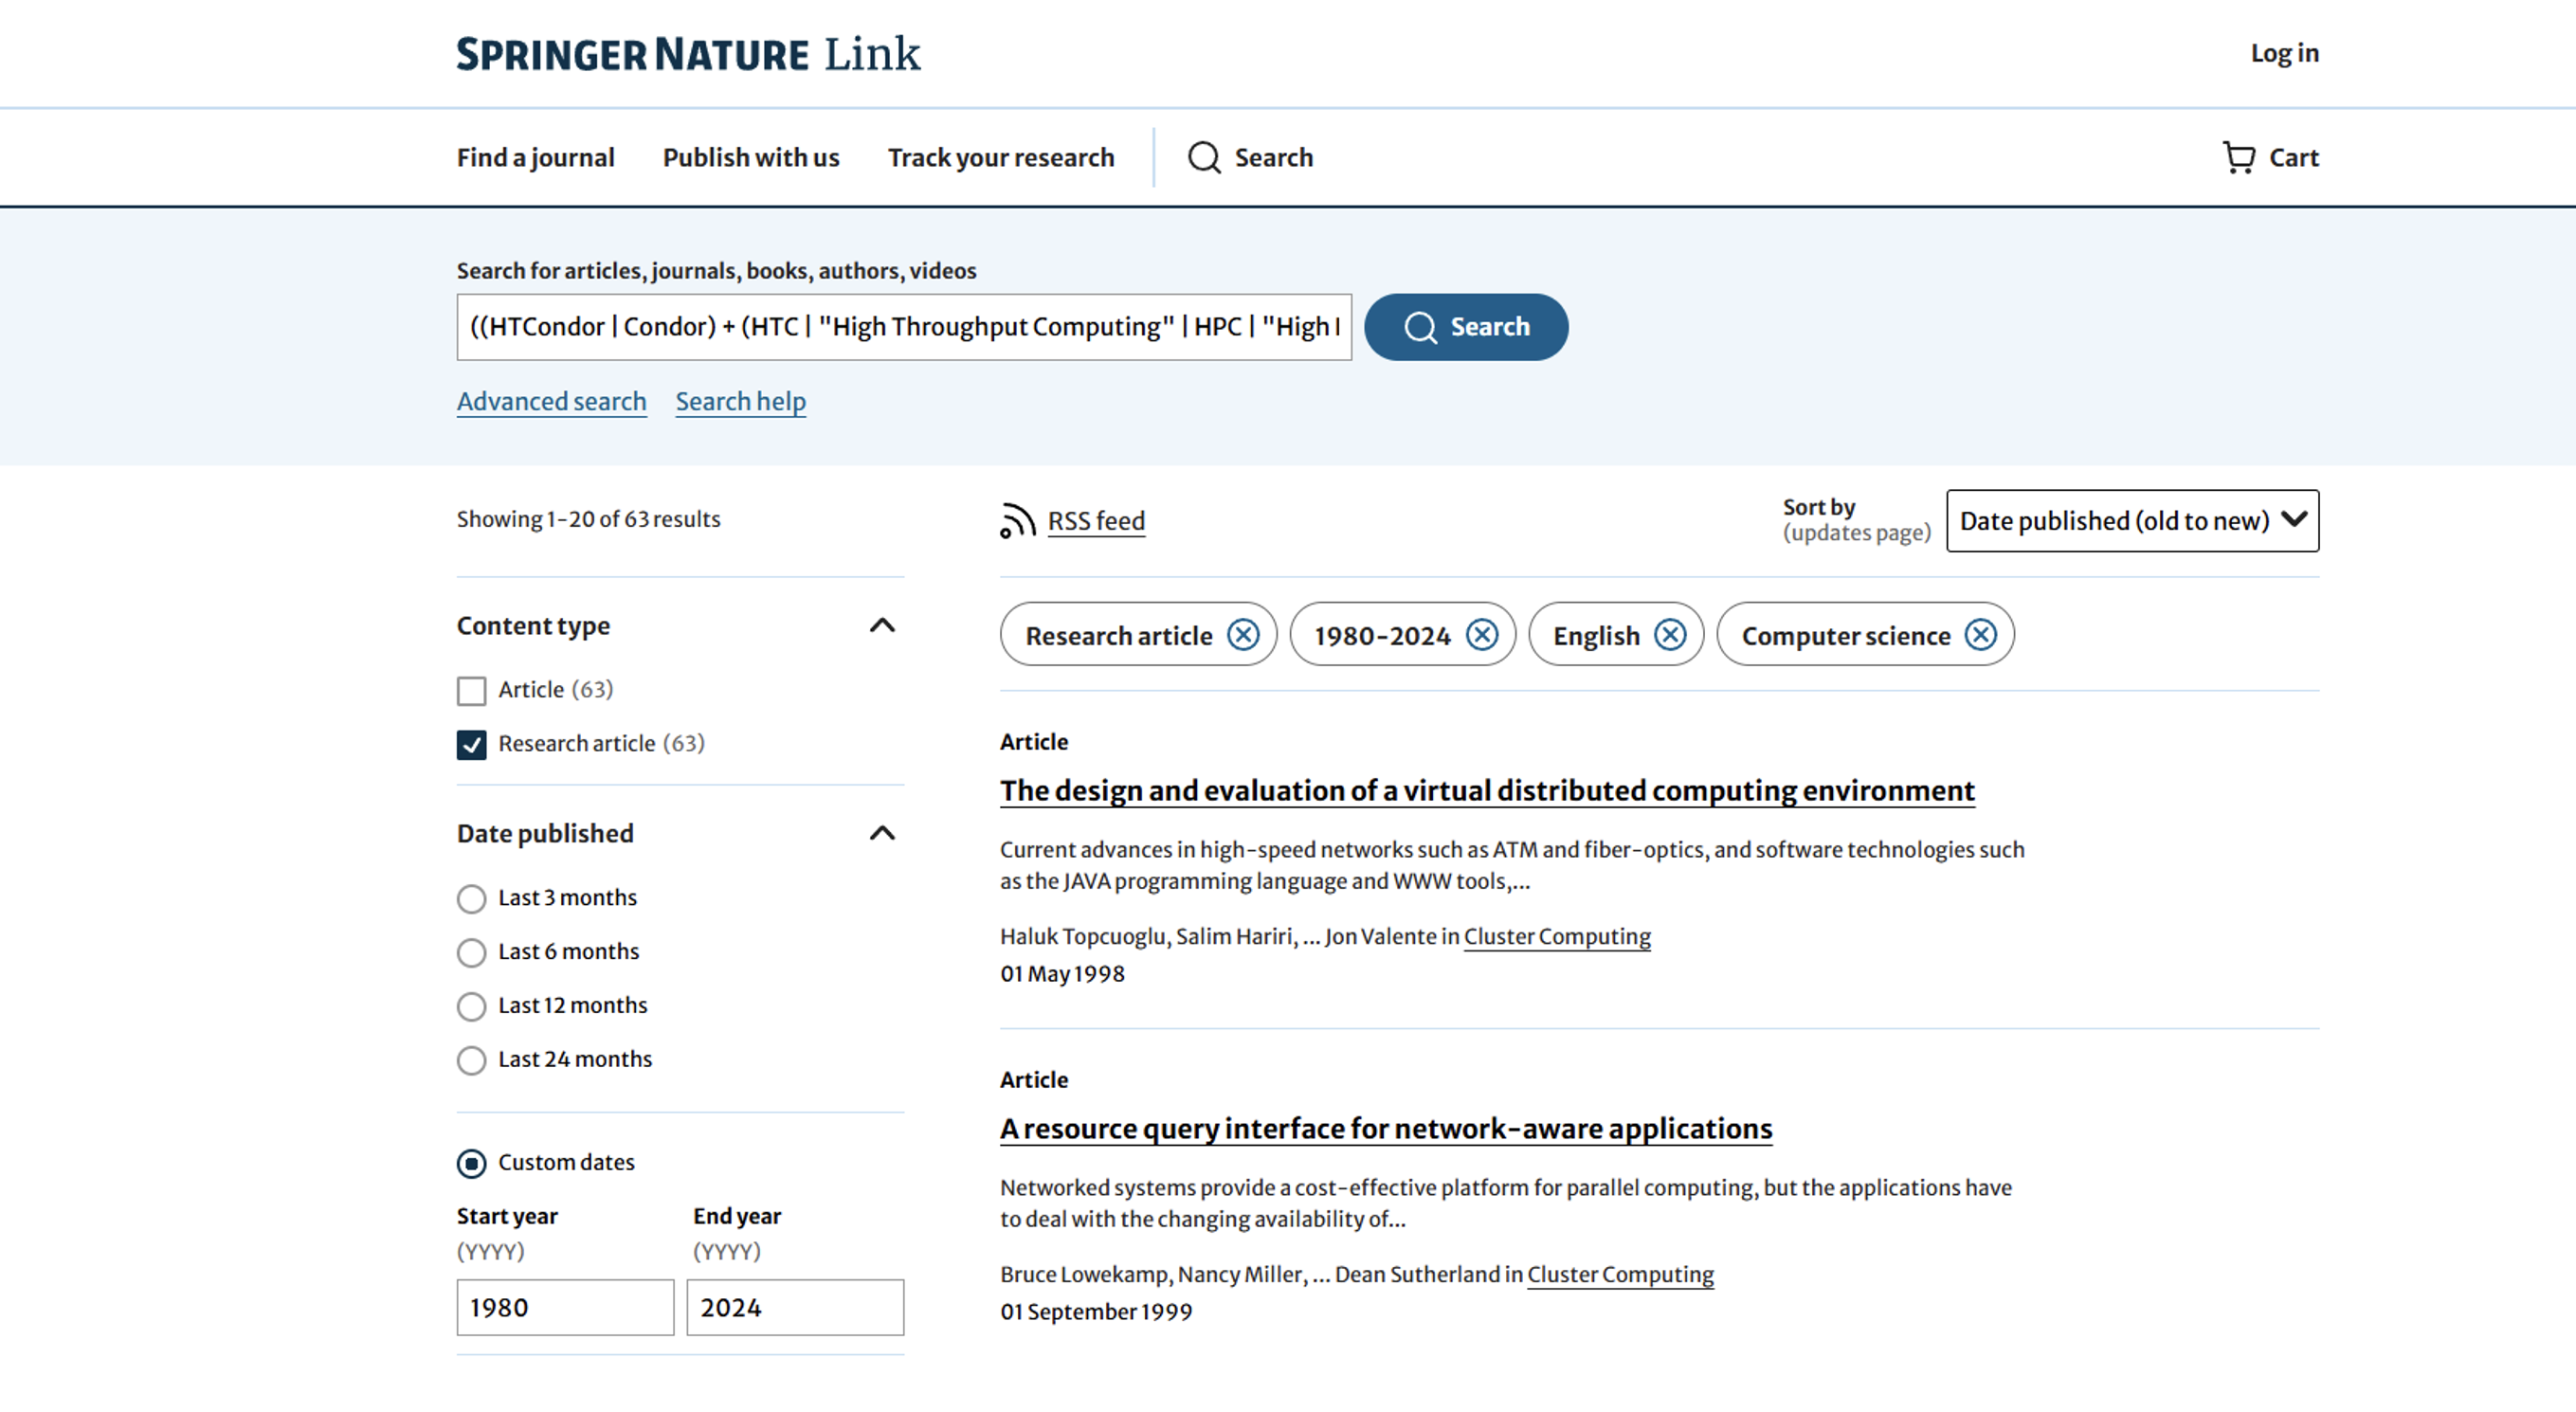
\includegraphics[width=\textwidth,keepaspectratio]{apendices/bases-datos/con-exclusion/springer.png}
	\caption{Búsqueda de artículos de investigación en ACM sin criterios de inclusión/exclusión \\
		Fecha de acceso: 12/03/25 8:23 pm
	}\label{fig:busqueda-springer-con-exclusion}
\end{figure}
